\documentclass{article}
\usepackage{graphicx, amssymb}
\usepackage{amsmath}
\usepackage{amsfonts}
\usepackage{amsthm}
\usepackage{kotex}
\usepackage{bm}
\usepackage{hyperref}
\usepackage{xcolor}
\usepackage{mathrsfs}
\usepackage{mathtools}
\usepackage{physics}
\usepackage{tikz}
\usetikzlibrary{decorations.markings}

\textwidth 6.5 truein 
\oddsidemargin 0 truein 
\evensidemargin -0.50 truein 
\topmargin -.5 truein 
\textheight 8.5in

\DeclareMathOperator{\cc}{\mathbb{C}}
\DeclareMathOperator{\rr}{\mathbb{R}}
\DeclareMathOperator{\bA}{\mathbb{A}}
\DeclareMathOperator{\fra}{\mathfrak{a}}
\DeclareMathOperator{\frb}{\mathfrak{b}}
\DeclareMathOperator{\frm}{\mathfrak{m}}
\DeclareMathOperator{\frp}{\mathfrak{p}}
\DeclareMathOperator{\slin}{\mathfrak{sl}}
\DeclareMathOperator{\Lie}{\mathsf{Lie}}
\DeclareMathOperator{\Alg}{\mathsf{Alg}}
\DeclareMathOperator{\Spec}{\mathrm{Spec}}
\DeclareMathOperator{\End}{\mathrm{End}}
\DeclareMathOperator{\rad}{\mathrm{rad}}
\newcommand*\Laplace{\mathop{}\!\mathbin\bigtriangleup}
\newcommand{\id}{\mathrm{id}}
\newcommand{\Hom}{\mathrm{Hom}}
\newcommand{\Sch}{\mathbf{Sch}}
\newcommand{\Ring}{\mathbf{Ring}}
\newcommand{\T}{\mathcal{T}}
\newcommand{\B}{\mathcal{B}}
\newcommand{\Mod}[1]{\ (\mathrm{mod}\ #1)}
\newtheorem{lemma}{Lemma}
\newtheorem{theorem}{Theorem}
\newtheorem{proposition}{Proposition}

\begin{document}
\title{Complex Analysis - HW3}
\author{SungBin Park, 20150462} 

\maketitle
\begin{enumerate}
\item[1.] Prove that $\int_{H_\epsilon} \frac{t^{z-1}}{e^t-1}dt$ is entire for $\epsilon<2\pi$, where $H_\epsilon$ is Hankel contour as Fig. \ref{Fig:P1}.
\begin{proof}
I'll use Morera's theorem. Let $\gamma$ be a closed piecewise $C^1$ curve in $\mathbb{C}$. Then,
\begin{equation*}
\int_\gamma \int_{H_\epsilon} \frac{t^{z-1}}{e^t-1}~dtdz = \int_{H_\epsilon}\frac{1}{e^t-1} \int_\gamma t^{z-1}~dz dt=\int_{H_\epsilon}0~dt=0
\end{equation*}
since $t^{z-1}$ is entire in $\mathbb{C}$.($\because \pdv{t^{z-1}}{\bar{z}}=0$.) By Morera's theorem, $\int_{H_\epsilon} \frac{t^{z-1}}{e^t-1}~dt$ is entire in $\mathbb{C}$.

Let's see why we can exchange integral. First, let's divide $H_\epsilon$ by $C_\epsilon$, $x:\infty\sim \delta(\epsilon)$, $x:\delta(\epsilon)\sim\infty $ where $\delta(\epsilon)$ is defined for connecting the straight lines and $C_\epsilon$. Assume the straight line have imaginary part $\sigma>0$. Then, $\frac{t^{z-1}}{e^t-1}$ is continuous on the contour.
\begin{equation*}
\begin{split}
\int_\gamma \int_{H_\epsilon} \frac{t^{z-1}}{e^t-1}~dtdz &= \int_\gamma\left( \int_{C_\epsilon} \frac{t^{z-1}}{e^t-1}~dt+\int_{\delta}^\infty \frac{(x-i\sigma)^{z-1}}{e^{x-i\sigma}-1}~dx+\int_\infty^\delta \frac{(x+i\sigma)^{z-1}}{e^{x+i\sigma}-1}~dt\right)dz.
\end{split}
\end{equation*}
For $z=a+bi$, $\abs{(x\pm i\sigma)^{z-1}}=\abs{e^{(a-1+bi)\log(x\pm i\sigma)}}\leq \abs{e^{(a-1)\log(\sqrt{x^2+\sigma^2})+\abs{b\theta}}}\leq 2\sqrt{x^2+\sigma^2}^{a-1}$ for sufficiently large $x$, where $\theta=\arg(x\pm i\sigma)$, so
\begin{equation*}
\abs{\int_{\delta}^\infty \frac{(x\pm i\sigma)^{z-1}}{e^{x\pm i\sigma}-1}~dx}\leq \abs{\int_{\delta}^R \frac{(x\pm i\sigma)^{z-1}}{e^{x\pm i\sigma}-1}~dx}+\int_{R}^\infty \frac{2\sqrt{x^2+\sigma^2}^{a-1}}{e^x-1}~dx<\infty
\end{equation*}
for sufficiently large $R$.
and it means $\frac{t^{z-1}}{e^t-1}$ is integrable on each domain. Therefore, we can use Fubini theorem and yield
\begin{equation*}
\int_\gamma \int_{H_\epsilon} \frac{t^{z-1}}{e^t-1}~dtdz = \int_{H_\epsilon}\frac{1}{e^t-1} \int_\gamma t^{z-1}~dz dt.
\end{equation*}
\end{proof}
\begin{figure}[h]
\centering
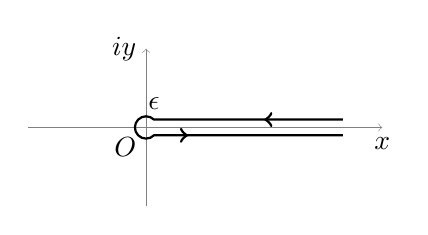
\begin{tikzpicture}[decoration={markings,
mark=at position 1cm with {\arrow[line width=1pt]{>}},
mark=at position 3.5cm with {\arrow[line width=1pt]{>}},
mark=at position 6.1cm with {\arrow[line width=1pt]{>}}
}
]
% The axes
\draw[help lines,->] (-1.5,0) -- (3,0) coordinate (xaxis);
\draw[help lines,->] (0,-1) -- (0,1) coordinate (yaxis);

% The path
\path[draw,line width=0.8pt,postaction=decorate] (2.5,0.1) -- (0.1,0.1) node[above] {$\epsilon$} arc (45:315:0.141421) -- (2.5,-0.1);


% The labels
\node[below] at (xaxis) {$x$};
\node[left] at (yaxis) {$iy$};
\node[below left] {$O$};
\end{tikzpicture}
\caption{Hankel Contour for $\epsilon<2\pi$. The branch cut is $\text{Re}\geq0$, $\text{Im}=0$.}
\label{Fig:P1}
\end{figure}
\newpage
\item[2.] Prove that $\zeta(s)\neq 0$ for $\Re s=0$.
\begin{proof}
I'll use the functional equation:
\begin{equation}\label{Eq:2}
\zeta(1-s)=2^{1-s}\pi^{-s}\cos\frac{\pi s}{2}\cdot \Gamma(s)\zeta(s).
\end{equation}
Put $s=1+it$ for $t\in \rr$, then
\begin{equation*}
\zeta(-it)=2^{-it}\pi^{-1-it}\cos\frac{\pi (1+it)}{2}\cdot \Gamma(1+it)\zeta(1+it).
\end{equation*}
If $t=0$, problem 3 proves that $\zeta(0)\neq 0$, so I'll assume that $t\neq 0$.
For $t\neq 0$, $\cos\frac{\pi (1+it)}{2}=\frac{i}{2}\left(e^{-\pi t/2}-e^{\pi t/2}\right)\neq 0$. Using identity
\begin{equation*}
\Gamma(s)\Gamma(1-s)=\frac{\pi}{\sin \pi s},
\end{equation*}
$\Gamma(-it)\Gamma(1+it)=\frac{\pi}{\sin \pi i t}$ and $\sin \pi i t< \infty$. Also, $\abs{\Gamma(it)}<\infty$ since $1/\Gamma(s)$ only have zeros in $0$, $-1$, $\cdots$. Therefore, $\Gamma(1+it)\neq 0$ for $t\in \rr\setminus\{0\}$. In the class, we proved that $\zeta(s)\neq 0$ at $\text{Re }s=1$. Hence,
\begin{equation*}
\zeta(it)\neq 0~~\text{for }t\in\rr.
\end{equation*}
\end{proof}
\item[3.] Prove that $\zeta(0)=-1/2$.
\begin{proof}
I'll use \eqref{Eq:2}. We know that $\zeta$ has a simple pole at $s=1$ and the residue is $1$. Therefore,
\begin{equation*}
\lim\limits_{s\rightarrow 1} \zeta(1-s)=\lim\limits_{s\rightarrow 1}2^{1-s}\pi^{-s}\cos\frac{\pi s}{2}\cdot \Gamma(s)\zeta(s)=\lim\limits_{s\rightarrow 1} 2^{1-s}\pi^{-s}\left(\frac{\pi}{2}-\frac{\pi}{2}s\right)\Gamma(s)\zeta(s)=-\frac{1}{2}\Gamma(1),
\end{equation*}
and $\Gamma(1)=1$. Therefore, $\lim\limits_{s\rightarrow 1}\zeta(1-s)$ exists and $\zeta(0)=-1/2$ since $\zeta(s)$ is entire except $s=1$.
\end{proof}
\end{enumerate}

\end{document}
